% vim: ts=4 sts=4 sw=4 et tw=75
\chapter{Algorithms and Data Structures}
\label{chap:alds}
\begin{quote}
    In the end, only familiarity with the tools and techniques of the field
    will provide right solution for a particular problem, and only a
    certain amount of experience will provide consistently professional
    result.
\end{quote}
\begin{quotesrc}
    Raymond Fielding.\bookname{The Technique of Special Effects
    Cinematography}
\end{quotesrc}
The study of algorithms and data structures is one of the foundations of
computer science, a rich field elegant techniques and sophisticated
mathematical analyses. And it's more than just fun and games for the
theoretically inclined: a good algorithm or data structure might make it
possible to solve a problem in seconds that could otherwise take years.

In specialized areas like graphics, databases, parsing, numerical analysis,
and simulation, the ability to solve problems depends critically on
state-of-the-artalgorithms and data structures. If you are developing your
programs in a field that's new to you, you \textit{must} find out what is
already known, lest (免得) you waste your time doing poorly what others have
already done well.

Every program depends on algorithms and data structures, but few programs
depend on the invention of brand new ones. Even within an intricate
(错综复杂的) program like a compiler or a web browser, most of the data
structures are arrays, lists, trees and hash tables. When a program needs
something more elaborate(详细), it will likely be based on these simpler
ones. Accordingly, for most programmers, the task is to know what
appropriate algorithms and data structures are available and to understand
how to choose among alternatives.

Here is the story in a nutshell. There are only a handful of basic
algorithms that show up in almost every program -- primarily searching and
sorting -- and even those are often included in libraries. Similarly,
almost every data structure is derived from a few fundamental ones. Thus
the material covered in this chapter will be familiar to almost all
programmers. We have written working versions to make the discussion
concrete, and you can lift code verbatim (逐字的) if necessary, but do so
only after you have investigated what the programming language and its
libraries have to offer.

\section{Searching}
Nothing beats an array for storing static tabular data. Compile-time
initialization makes it cheap and easy to construct such arrays. (In Java,
the initialization occurs at run-time, but this is an unimportant
implementation detail unless the arrays are large.) In a program to detect
words that are used rather too much in bad prose, we can write
\begin{wellcode}
    /* lookup: sequential search for word in array */
    int lookup(char *word, char *array[])
    {
        int i;
        for (i = 0; array[i] != NULL; i++)
           if (strcmp(word, array[i] == 0))
                return i;
        return -1;
    }
\end{wellcode}
In C and C++, a parameter that is an array of strings can be declared as
\verb"char *array[]" or \verb"char *+array". Although these forms are
equivalent, the first makes it clearer how the parameter will be used.

This search algorithm is called \textbf{\textit{sequential search}} because
it looks at each element in turn to see if it's the desired one. When the
amount of data is small, sequential search is fast enough. There are
standard library routines to do sequential search for specific data types;
for example, functions like \texttt{strchr} and \texttt{strstr} search for
the first instance of a given character or substring in a C or C++ string.
The Java \verb'String' class has an \verb'indexOf' method, and the generic
C++ \verb'find' algorithms apply to most data types. If such a function
exists for the data type you've got, use it.

Sequential search is easy but the amount of work is directly proportional
to the amount of data to be searched; doubling the number of elements will
double the time to search if the desired item is not present. This is a
linear relationship -- run-time is a linear function of data size -- so
this method is also known as \textbf{\textit{linear search}}.


Here's an excerpt from an array of more realistic size from a program that
parses HTML, which defines textual names for well over a hundred individual
characters:
\begin{wellcode}
    typedef struct Nameval Nameval;
    struct Nameval{
        char *name;
        int value;
    };
    /* HTML characters, e.g. AElig is ligature of A and E. */
    /* Values are Unicode/ISO10646 encoding. */
    Nameval htmlchars[] = {
        "AElig",    0x00c6,
        "Aacute",   0x00c1,
        "Acirc",    0x00c2,
        /* ... */
        "zeta",     0x03b6,
    };
\end{wellcode}
For a larger array like this, it's more efficient to use
\textit{binary} search. The binary search algorithm is an orderly
version of the way we look up words in a dictionary. Check the middle
element. If that value is bigger than what we are looking for, look in the
first half; otherwise, look in the second half. Repeat until the desired
item is found or determined not to be present.

For binary search, the table must be sorted, as it is here (that's good
style anyway; people find things faster in sorted tables too), and we must
know how long the table is. The \verb'NELEMS' macro from Chapter
\ref{chap:style} can
help:
\begin{wellcode}
    printf("The HTML table has %d words\n", NELEMS(htmlchars));
\end{wellcode}

A binary search function for this table might look like this:
\begin{wellcode}
    /* lookup: binary search for name in tab; return index */
    int lookup(char *name, NameVal tab[], int ntab)
    {
        int low, high, mid, cmp;
        low = 0;
        high = ntab - 1;
        while(low <= high){
            mid = (low + high)/2;
            cmp = strcmp(name, tab[mid].name);
            if(cmp < 0){
                high = mid - 1;
            }
            else if(cmp > 0){
                low = mid + 1;
            }
            else{   /* found match */
                return mid;
            }
        }
        return -1;  /* no match */
    }
\end{wellcode}
Putting all this together, to search \verb'htmlchars' we write
\begin{wellcode}
    half = lookup("frac12", htmlchars, NELEMS(htmlchars));
\end{wellcode}
to find the array index of the character $1/2$.

Binary search eliminates half the data at each step. The number of steps is
therefore proportional to the number of times we can divide $n$ by 2
before we're left with a single element. Ignoring roundoff, this is $\log_2
n$. If we have 1000 items to search, linear search takes up to 1000 steps,
while binary search takes about 10; if we have a million items. linear
takes a million steps and binary takes 20. The more items, the greater the
advantage of binary search. Beyond some size of input (which varies with
the implementation), binary search is faster than linear search.

\section{Sorting}
Binary search works only if the elements are sorted. If repeated searches
are going to be made in some data set, it will be profitable to sort once
and then use binary search. If the data set is known in advance, it can be
sorted when the program is written and built using compile-time
initialization. If not, it must be sorted when the program is run.

One of the best all-round sorting algorithms is quicksort, which was
invented in 1960 by C. A. R. Hoare. Quicksort is a fine example of how to
avoid extra computing. It works by partitioning an array into little and
big elements:                                                           \\
\indent pick one element of the array (the "pivot").                    \\
\indent partition the other elements into two groups:                   \\
\indent \indent "little ones" that are less than the pivot value, and   \\
\indent \indent "big ones" that are greater than or equal to the pivot
value.                                                                  \\
\indent recursively sort each group.                                    \\
When this process is finished, the array is in order. Quicksort is fast
because once an element is known to be less than the pivot value, we don't
have to compare it to any of the big ones; similarly. big ones are not
compared to little ones. This makes it much faster than the simple sorting
methods such as insertion sort and bubble sort that compare each element
directly to all the others.

Quicksort is practical and efficient; it has been extensively studied and
myriad variations exist. The version that we present here is just about the
simplest implementation but it is certainly not the quickest.

This \verb'quicksort' function sorts an array of integers:
\begin{wellcode}
    /* quicksort: sort v[0]..v[n-1] into increasing order */
    void quicksort(int v[], int n)
    {
        int i, last;
        if(n <= 1) /* nothing to do */
        {
            return;
        }
        swap(v, 0, rand() % n); /* move pivot elem to v[0] */
        last = 0;
        for(i = 1; i < n; i++)  /*partition */
        {
            if(v[i] < v[0])
            {
                swap(v, ++last, i);
            }
            swap(v, 0, last);   /* restore pivot */
            quicksort(v, last); /* recursively sort */
            quicksort(v + last + 1, n - last - 1); /* each part */
        }
    }
\end{wellcode}

The \verb'swap' operation, which interchanges two elements, appears three
times in quicksort, so it is best made into a separate function:
\begin{wellcode}
    /* swap: interchange v[i] and v[j] */
    void swap(int v[], int i, int j)
    {
        int temp;
        temp = v[i];
        v[i] = v[j];
        v[j] = temp;
    }
\end{wellcode}

Partitioning selects a random element as the pivot. swaps it temporarily to
the front, then sweeps through the remaining elements, exchanging those
smaller than the pivot ("little ones") towards the beginning (at location
\verb'lastr') and big ones towards At the beginning of the process, just
after the pivot has been the end (at location \verb'i').  swapped to the
front, \verb'last = 0' and elements \verb'i = 1' through \verb'n-1' are
unexamined:
\begin{figure}[h]
    \centering
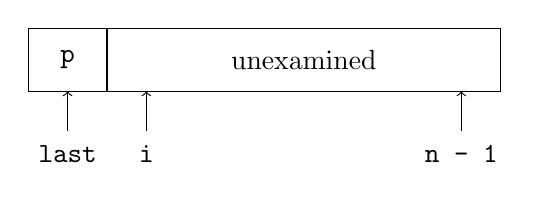
\begin{tikzpicture}
    \draw (0, 0) -- (6, 0);
    \draw (0, 0.8) -- (6, 0.8);
    \draw (0, 0) -- (0, 0.8);
    \draw (1, 0) -- (1, 0.8);
    \draw (6, 0) -- (6, 0.8);
    \node at(0.5, 0.4) {\texttt{p}};
    \node at(3.5, 0.4) {unexamined};
    \draw[->] (0.5, -0.5) -- (0.5, 0);
    \draw[->] (1.5, -0.5) -- (1.5, 0);
    \draw[->] (5.5, -0.5) -- (5.5, 0);
    \node at(0.5, -0.8) {\texttt{last}};
    \node at(1.5, -0.8) {\texttt{i}};
    \node at(5.5, -0.8) {\texttt{n - 1}};
\end{tikzpicture}
\end{figure}
